\chapter{KAJIAN PUSTAKA}

\section{Penelitian Terdahulu}

Penelitian ini mengintegrasikan ekstraksi informasi terstruktur dengan metode pencarian hibrida. Rangkuman studi terdahulu yang melandasi penelitian ini disajikan pada \ref{tab:penelitian_terdahulu_revisi}.

\renewcommand{\arraystretch}{1.3}
\begin{longtable}{|p{4cm}|p{2cm}|p{10cm}|}
    \caption{Tinjauan Penelitian Terdahulu} \label{tab:penelitian_terdahulu_revisi}                                                                                          \\

    \hline
    \textbf{Judul}                                                                                                                  & \textbf{Penulis} & \textbf{Kesimpulan} \\ \hline
    \endfirsthead

    \hline
    \textbf{Judul}                                                                                                                  & \textbf{Penulis} & \textbf{Kesimpulan} \\ \hline
    \endhead

    \hline
    \multicolumn{3}{r}{\textit{Bersambung ke halaman berikutnya...}}                                                                                                         \\
    \endfoot

    \hline
    \endlastfoot

    % --- Studi 1 ---
    \textit{Swamped with Too Many Articles: GraphRAG Makes Getting Started Easy}                                                    &
    \cite{Ngangmeni2025SwampedWT}                                                                                                   &
    Evaluasi komparatif menunjukkan bahwa \textit{GraphRAG} mengungguli \textit{Naive RAG} dan \textit{LightRAG} dalam empat metrik kritis: \textbf{\textit{Comprehensiveness, Diversity, Empowerment,}} dan \textbf{\textit{Directness}}. Temuan ini memvalidasi landasan penelitian bahwa pendekatan berbasis graf menawarkan navigasi semantik yang lebih superior dibandingkan pencarian leksikal untuk mengatasi \textit{literature overload} pada repositori data berskala besar.
    \\ \hline
    % --- Studi 2 ---
    \textit{HybridRAG: Integrating Knowledge Graphs and Vector Retrieval Augmented Generation for Efficient Information Extraction} &
    \cite{10.1145/3677052.3698671}                                                                                                  &
    Penelitian ini menetapkan standar efektivitas arsitektur hibrida dengan pencapaian skor \textbf{\textit{Faithfulness} dan \textit{Answer Relevance} sebesar 0,96} serta \textbf{\textit{Context Recall} sempurna (1,00)}. Hasil empiris ini menjadi rujukan utama penelitian usulan, yang membuktikan bahwa penggabungan \textit{Knowledge Graph} dan \textit{Vector Retrieval} adalah strategi optimal untuk memitigasi halusinasi dan memaksimalkan presisi jawaban pada dokumen kompleks.
    \\ \hline
    % --- Studi 3 ---
    \textit{Knowledge Graph Generation and Application for Unstructured Data Using Data Processing Pipeline}                        &
    \cite{thushara2024}                                                                                                             &
    Mengembangkan \textit{pipeline} otomatis menggunakan model generatif \textit{REBEL} yang mencapai \textbf{akurasi ekstraksi 87\%} pada data tidak terstruktur. Metrik akurasi ini menyoroti tantangan yang ada, yang dalam penelitian ini akan ditingkatkan melalui strategi \textit{Parallel Processing} (integrasi data terstruktur PDDikti/SINTA dan teks abstrak) untuk melampaui batasan akurasi model generatif tunggal dalam konstruksi KG.
    \\ \hline
\end{longtable}

\section{Kajian Teori}

\subsection{\textit{Scholarly Search}}

\textit{Scholarly search} atau pencarian literatur akademik berfokus pada pengelolaan dan pengambilan dokumen ilmiah dari repositori besar, mencakup artikel jurnal, prosiding, tesis, serta metadata terkait \citep{Kasela_2025}. Saat ini, domain ini menghadapi tantangan \textit{literature overload}. \citet{Larsen2010} melaporkan bahwa volume publikasi di beberapa bidang berlipat ganda setiap 8 hingga 15 tahun. Dengan lebih dari 200 juta artikel tersedia, peneliti menanggung beban kognitif (\textit{cognitive overload}) yang berat saat mencari referensi secara manual.

Sistem pencarian tradisional seperti \textit{Google Scholar}, \textit{PubMed}, dan \textit{CiteSeerX} memiliki keterbatasan karena mengandalkan sinyal leksikal murni seperti algoritma \textit{BM25} \citep{10.1007/s11192-020-03690-4}. Pendekatan leksikal tersebut seringkali gagal menangkap hubungan makna kompleks antar konsep, kesulitan mengenali sinonim, dan mengabaikan relasi konektivitas antar dokumen. Akibatnya, hasil pencarian sering berupa daftar panjang dokumen yang harus diverifikasi manual oleh peneliti, tanpa indikasi relevansi langsung terhadap pertanyaan riset.

Dokumen ilmiah memiliki karakteristik unik yang membedakannya dari teks biasa. \citet{Shen2016ModelingTA} menyebutkan bahwa dokumen ilmiah terdiri dari dua dimensi utama: dimensi tekstual (isi dan metadata) serta struktural (jejaring sitasi, ko-sitasi, dan kolaborasi). Keberhasilan pencarian ilmiah di masa depan tidak hanya bergantung pada kemiripan vektor teks (\textit{vector proximity}), tetapi juga pada kemampuan penalaran relasional (\textit{relational reasoning}). Sebagai contoh, \citet{avgoren2025enhancing} menunjukkan bahwa pendekatan relasional mampu menghubungkan metodologi dari satu makalah dengan temuan di makalah lain melalui mekanisme \textit{multi-hop reasoning}.

Dalam implementasi praktis, \citet{9522111} menjelaskan bahwa \textit{scholarly search} telah berkembang menjadi beragam tugas spesifik, mulai dari pencarian berbasis topik, penelusuran sitasi, rekomendasi artikel, hingga \textit{question answering} berbasis literatur. Kompleksitas tugas-tugas tersebut menuntut sistem pencarian yang mampu mengintegrasikan berbagai jenis sinyal semantik dan hubungan struktural antar dokumen secara simultan.

Perkembangan terkini, sebagaimana dicatat oleh \citet{gupta2024comprehensivesurveyretrievalaugmentedgeneration}, menunjukkan pemanfaatan \textit{scholarly search} dalam sistem \textit{question answering}. Sistem ini dituntut tidak hanya menampilkan dokumen, tetapi juga menyajikan wawasan lintas bidang, mengidentifikasi celah riset (\textit{research gaps}), dan menyediakan bukti sumber informasi (\textit{traceability}). Urgensi presisi fakta dan navigasi relasional inilah yang mendasari integrasi teknologi \textit{Knowledge Graph} dan \textit{Large Language Models} dalam penelitian ini.

\subsection{\textit{Knowledge Graph}}

\textit{Knowledge base} adalah kumpulan data terorganisir yang mendeskripsikan entitas dan hubungannya dalam format \textit{triplet}. Ketika himpunan \textit{triplet} ini direpresentasikan sebagai jaringan dengan entitas sebagai titik (\textit{node}) dan hubungan sebagai garis (\textit{edge}), strukturnya disebut \textit{Knowledge Graph} \citep{mondal2021end}. Berbeda dengan basis data relasional yang kaku, \textit{Knowledge Graph} menawarkan representasi pengetahuan yang dinamis. Struktur graf ini memungkinkan mesin memahami hubungan antar potongan informasi, menyerupai mekanisme asosiasi kognitif manusia \citep{cheng2025humancognitioninspiredrag}.

Komponen fundamental dari sebuah \textit{Knowledge Graph} adalah \textit{triplet} faktual yang terdiri dari \textit{Subjek-Predikat-Objek} atau \textit{Head-Relation-Tail}. \textit{Knowledge Graph} menyimpan pengetahuan terstruktur sebagai himpunan \textit{triplet}, yang dapat direpresentasikan sebagai berikut:

\begin{equation}
    G = (E, R, T)
    \label{eq:kg-definition}
\end{equation}
di mana $E$ adalah himpunan entitas (seperti individu atau objek), $R$ adalah himpunan relasi (seperti ``bagian\_dari''), dan $T$ adalah himpunan \textit{triplet} yang membentuk keseluruhan struktur graf tersebut \citep{Hogan_2021}. Setiap elemen di dalam $T$ merepresentasikan satu fakta tunggal yang diformulasikan sebagai:

\begin{equation}
    (h, r, t) \in T
    \label{eq:triplet-format}
\end{equation}
di mana $h$ adalah entitas sumber atau \textit{head}, $t$ adalah entitas tujuan atau \textit{tail}, dan $r$ adalah relasi yang menghubungkan keduanya \citep{peng2023knowledge}. Contohnya dalam konteks akademik
\begin{itemize}
    \item $(\underbrace{\text{\texttt{Dosen\_A}}}_{\text{head}}) \xrightarrow{\underbrace{\text{\small menulis}}_{\text{relation}}} (\underbrace{\text{\texttt{Publikasi\_B}}}_{\text{tail}})$
    \item $(\underbrace{\text{\texttt{Publikasi\_B}}}_{\text{head}}) \xrightarrow{\underbrace{\text{\small mensitasi}}_{\text{relation}}} (\underbrace{\text{\texttt{Publikasi\_C}}}_{\text{tail}})$
    \item $(\underbrace{\text{\texttt{Dosen\_A}}}_{\text{head}}) \xrightarrow{\underbrace{\text{\small berafiliasi\_dengan}}_{\text{relation}}} (\underbrace{\text{\texttt{Universitas\_X}}}_{\text{tail}})$
\end{itemize}
Struktur ini sangat efektif karena arah panah memberi makna eksplisit, di mana entitas \textit{head} menunjuk langsung ke entitas \textit{tail} melalui garis relasi (\textit{edge}). Jika digambarkan sebagai graf, struktur ini akan terlihat seperti pada \ref{fig:simple-kg}.

\begin{figure}[htbp]
    \centering
    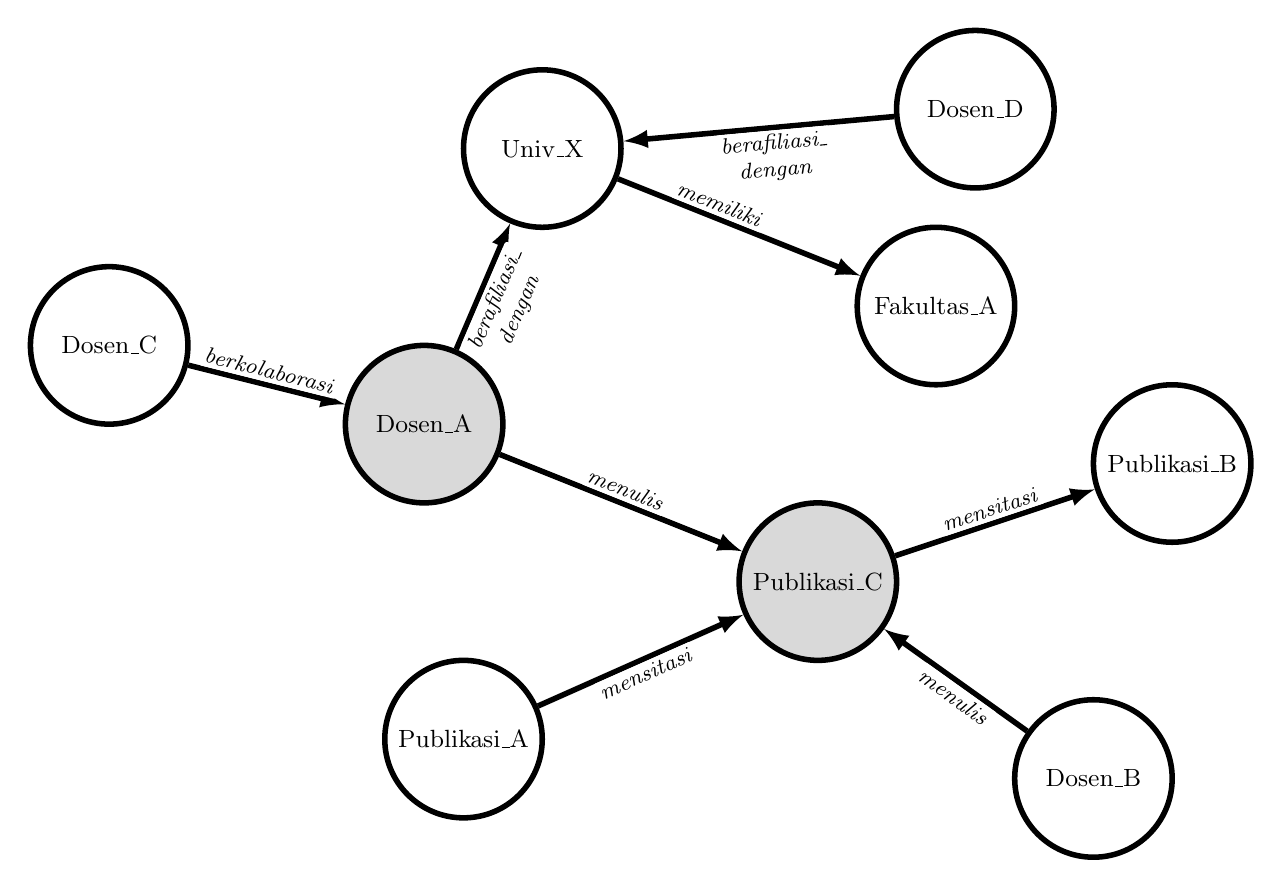
\begin{tikzpicture}[
            node distance=2cm,
            every node/.style={font=\small},
            entity/.style={circle, draw, line width=2pt, minimum size=2cm, align=center, inner sep=2pt},
            graynode/.style={entity, fill=gray!30},
            whitenode/.style={entity, fill=white},
            arrow/.style={->, >=latex, line width=2pt},
            lbl/.style={font=\footnotesize, fill=white, inner sep=1.5pt, rounded corners=1pt}
        ]

        % Nodes — spread wider to avoid label overlap
        \node[graynode] (dosen_a) at (0,0) {Dosen\_A};
        \node[graynode] (pub_c) at (5,-2) {Publikasi\_C};

        \node[whitenode] (dosen_c) at (-4,1) {Dosen\_C};
        \node[whitenode] (univ_x) at (1.5,3.5) {Univ\_X};

        \node[whitenode] (dosen_d) at (7,4) {Dosen\_D};
        \node[whitenode] (fak_a) at (6.5,1.5) {Fakultas\_A};

        \node[whitenode] (pub_b) at (9.5,-0.5) {Publikasi\_B};
        \node[whitenode] (pub_a) at (0.5,-4) {Publikasi\_A};
        \node[whitenode] (dosen_b) at (8.5,-4.5) {Dosen\_B};

        % === EDGES — all labeled ===

        % Dosen_C -> Dosen_A (berkolaborasi)
        \draw[arrow] (dosen_c) -- node[lbl, above, sloped] {\textit{berkolaborasi}} (dosen_a);

        % Dosen_A -> Univ_X (berafiliasi_dengan) — label below to avoid clash
        \draw[arrow] (dosen_a) -- node[lbl, below, sloped, pos=0.45, align=center] {\textit{berafiliasi\_}\\\textit{dengan}} (univ_x);

        % Univ_X -> Dosen_D (berafiliasi_dengan)
        \draw[arrow] (dosen_d) -- node[lbl, below, sloped, pos=0.45, align=center] {\textit{berafiliasi\_}\\\textit{dengan}} (univ_x);

        % Univ_X -> Fakultas_A (memiliki)
        \draw[arrow] (univ_x) -- node[lbl, above, sloped, pos=0.4] {\textit{memiliki}} (fak_a);

        % Dosen_A -> Pub_C (menulis)
        \draw[arrow] (dosen_a) -- node[lbl, above, sloped] {\textit{menulis}} (pub_c);

        % Pub_A -> Pub_C (mensitasi)
        \draw[arrow] (pub_a) -- node[lbl, below, sloped] {\textit{mensitasi}} (pub_c);

        % Pub_C -> Pub_B (mensitasi)
        \draw[arrow] (pub_c) -- node[lbl, above, sloped] {\textit{mensitasi}} (pub_b);

        % Pub_C -> Dosen_B (ditulis_oleh)
        \draw[arrow] (dosen_b) -- node[lbl, below, sloped, pos=0.45] {\textit{menulis}} (pub_c);

    \end{tikzpicture}
    \caption{Visualisasi \textit{Knowledge Graph} akademik yang menunjukkan relasi antar entitas.}
    \label{fig:simple-kg}
\end{figure}

Menurut \citet{Hofer_2024}, pengembangan \textit{Knowledge Graph} (KG) terbagi dalam dua paradigma utama: \textit{Resource Description Framework} (RDF) dan \textit{Labeled Property Graph} (LPG). Penelitian ini mengadopsi struktur \textit{LPG} (menggunakan \textit{Neo4j}) karena keunggulannya dalam navigasi hubungan kompleks dan fleksibilitas skema. Keunggulan fundamental \textit{KG} dibandingkan metode leksikal adalah kemampuan penalaran bertahap (\textit{multi-hop reasoning}), yang memungkinkan sistem menghubungkan entitas yang secara semantik terpisah namun memiliki keterkaitan logis, sebuah fitur vital untuk sintesis akademik.

Dalam lingkungan universitas, penerapan \textit{Scholarly Knowledge Graph} (SKG) memiliki peranan penting dalam mengatasi fenomena \textit{knowledge island} yang dijelaskan oleh \cite{YU201748}, yaitu kondisi di mana pengetahuan terisolasi, tidak saling terhubung, dan sulit diintegrasikan satu sama lain. \textit{SKG} didefinisikan sebagai representasi graf yang memodelkan entitas akademik (seperti penulis, publikasi, dan institusi) beserta hubungan antar mereka secara eksplisit. Dalam konteks kecerdasan buatan modern, \textit{Knowledge Graph} (KG) menjadi elemen penting dalam arsitektur \textit{Retrieval-Augmented Generation}, di mana struktur graf digunakan untuk menyediakan konteks faktual kepada \textit{LLM}, mengurangi risiko halusinasi, serta mendukung penalaran multi-langkah yang tidak dapat dicapai oleh metode pencarian konvensional.

\subsection{\textit{Knowledge Extraction}}
\textit{Knowledge Extraction} atau ekstraksi pengetahuan merupakan proses krusial untuk mentransformasi data tidak terstruktur (seperti teks naratif dalam publikasi ilmiah, email, atau dokumen PDF) menjadi representasi pengetahuan yang terorganisir, formal, dan dapat diolah oleh mesin \citep{WANG2018112}. Dalam ekosistem \textit{Knowledge Graph}, \textit{Knowledge Extraction} berperan dalam menyarikan fakta-fakta atomik dari teks untuk mengisi dan memperbarui struktur graf tersebut. Implementasi ini berfungsi sebagai fondasi untuk membangun basis pengetahuan (\textit{knowledge base}) yang dapat memfasilitasi mekanisme penalaran sistem dalam menghasilkan jawaban yang akurat.

Secara formal, tugas \textit{Knowledge Extraction} dapat diformulasikan sebagai fungsi pemetaan dari teks input \(\mathcal{T}\) menjadi representasi terstruktur \(\mathcal{S}\). Representasi ini terdiri dari himpunan entitas \(E\) dan relasi \(R\), sebagaimana dinyatakan dalam Persamaan \ref{eq:ie-mapping}:

\begin{equation}
    \mathcal{S} = f_{IE}(\mathcal{T}) = \{(e_i, r_{ij}, e_j) \mid e_i, e_j \in E, r_{ij} \in R\}
    \label{eq:ie-mapping}
\end{equation}
di mana setiap elemen dalam \(\mathcal{S}\) berupa \textit{triplet} \((e_i, r_{ij}, e_j)\) yang merepresentasikan satu fakta tunggal, dengan \(e_i\) bertindak sebagai entitas subjek, \(r_{ij}\) sebagai predikat atau relasi, dan \(e_j\) sebagai entitas objek.

Implementasi fungsi pemetaan berskala besar menuntut otomatisasi, mengingat ekstraksi manual tidak lagi memadai untuk menangani pertumbuhan volume data tekstual yang eksponensial \citep{Premasiri2025}. Secara umum, proses otomatisasi \textit{Knowledge Extraction} didekomposisi menjadi tiga tahapan fundamental:

\begin{enumerate}[label=\textbf{\arabic*.}, leftmargin=*, itemsep=10pt]
    \item \textbf{\textit{Named Entity Recognition} (NER)}

          \hspace*{0.75cm} Sebagai langkah awal, \textit{Named Entity Recognition} (NER) bertugas mengidentifikasi dan mengklasifikasikan entitas penting dalam teks untuk menemukan himpunan entitas \(E\) (Persamaan \ref{eq:ie-mapping}). NER mendeteksi istilah relevan seperti nama orang, organisasi, atau terminologi ilmiah, lalu memberikan label kategori yang sesuai \citep{ZHAO2023225}.

    \item \textbf{\textit{Relation Extraction} (RE)}

          \hspace*{0.75cm} \textit{Relation Extraction} (RE) bertujuan mengidentifikasi hubungan semantik (\(r_{ij}\)) antara dua entitas (\(e_i\) dan \(e_j\)) yang ditemukan. Proses ini mengklasifikasikan jenis interaksi yang terjadi, misalnya hubungan ``menggunakan'' antara metode dan algoritma, atau ``ditulis oleh'' antara publikasi dan peneliti.

    \item \textbf{\textit{Event Extraction} (EE)}

          \hspace*{0.75cm} Untuk memperkaya lapisan semantik, \textit{Event Extraction} (EE) kerap ditambahkan. Berbeda dengan RE yang memetakan hubungan statis, EE berfokus pada identifikasi peristiwa dinamis yang mencakup pemicu (\textit{trigger}) serta argumen pendukungnya (pelaku, waktu, lokasi).

\end{enumerate}

Secara metodologis, pendekatan ekstraksi pengetahuan telah berevolusi dari sistem berbasis aturan (\textit{rule-based systems}) dan analisis tata bahasa seperti \textit{dependency parsing} menuju penggunaan model \textit{Deep Learning} yang lebih kompleks, seperti arsitektur \textit{BERT} dan \textit{BiLSTM-CRF} \citep{han2025ragvsgraphragsystematic}. Pada paradigma kontemporer, penggunaan Model Bahasa Besar (\textit{Large Language Models}) telah menjadi standar baru melalui teknik \textit{zero-shot} dan \textit{few-shot prompting} untuk melakukan ekstraksi secara otomatis. \cite{sanmartin2024kgragbridginggapknowledge} membuktikan bahwa \textit{LLM} unggul dalam menangkap hubungan semantik yang bersifat implisit dan kaya akan konteks dibandingkan metode tradisional. Meskipun demikian, penggunaan \textit{LLM} dalam ekstraksi tetap memerlukan mekanisme validasi atau koreksi mandiri (\textit{self-correction}) untuk meminimalkan risiko kesalahan ekstraksi atau halusinasi informasi.

Dalam penelitian ini, efektivitas \textit{Knowledge Extraction} sangat berperan dalam menentukan kualitas pengambilan informasi. Proses ekstraksi yang mendalam terhadap kontribusi riset, seperti metode yang diajukan, dataset yang digunakan, serta metrik hasil, memungkinkan sistem untuk mengaitkan berbagai temuan ilmiah yang tersebar, mempermudah penemuan pola baru, serta memastikan bahwa setiap jawaban yang diberikan dapat ditelusuri kembali ke bukti asli dalam literatur (\textit{traceability}).

\subsection{\textit{Large Language Models} (LLM)}

\textit{Large Language Models} (\textit{LLM})  merepresentasikan kelas model \textit{Deep Learning} canggih yang dilatih menggunakan sejumlah besar data teks untuk memahami, memproses, dan menghasilkan teks dengan kualitas yang menyerupai bahasa manusia \citep{zhao2025surveylargelanguagemodels}. Secara struktural, mayoritas \textit{LLM} modern dibangun di atas arsitektur \textit{Transformer} yang memanfaatkan mekanisme \textit{self-attention} (\textit{multi-head attention}) dan \textit{feed-forward networks}, seperti ditunjukkan pada \ref{fig:transformer-arch} dan pertama kali diperkenalkan oleh \cite{NIPS2017_3f5ee243}. Mekanisme ini memungkinkan model untuk memproses seluruh urutan kata dalam suatu kalimat secara simultan dan menangkap ketergantungan jarak jauh (\textit{long-range dependencies}) antar kata, memberikan pemahaman konteks yang jauh lebih dalam dibandingkan model tradisional seperti \textit{RNN} atau \textit{LSTM} yang memproses data secara sekuensial.

\begin{figure}[!t]
    \centering
    \makebox[\textwidth][c]{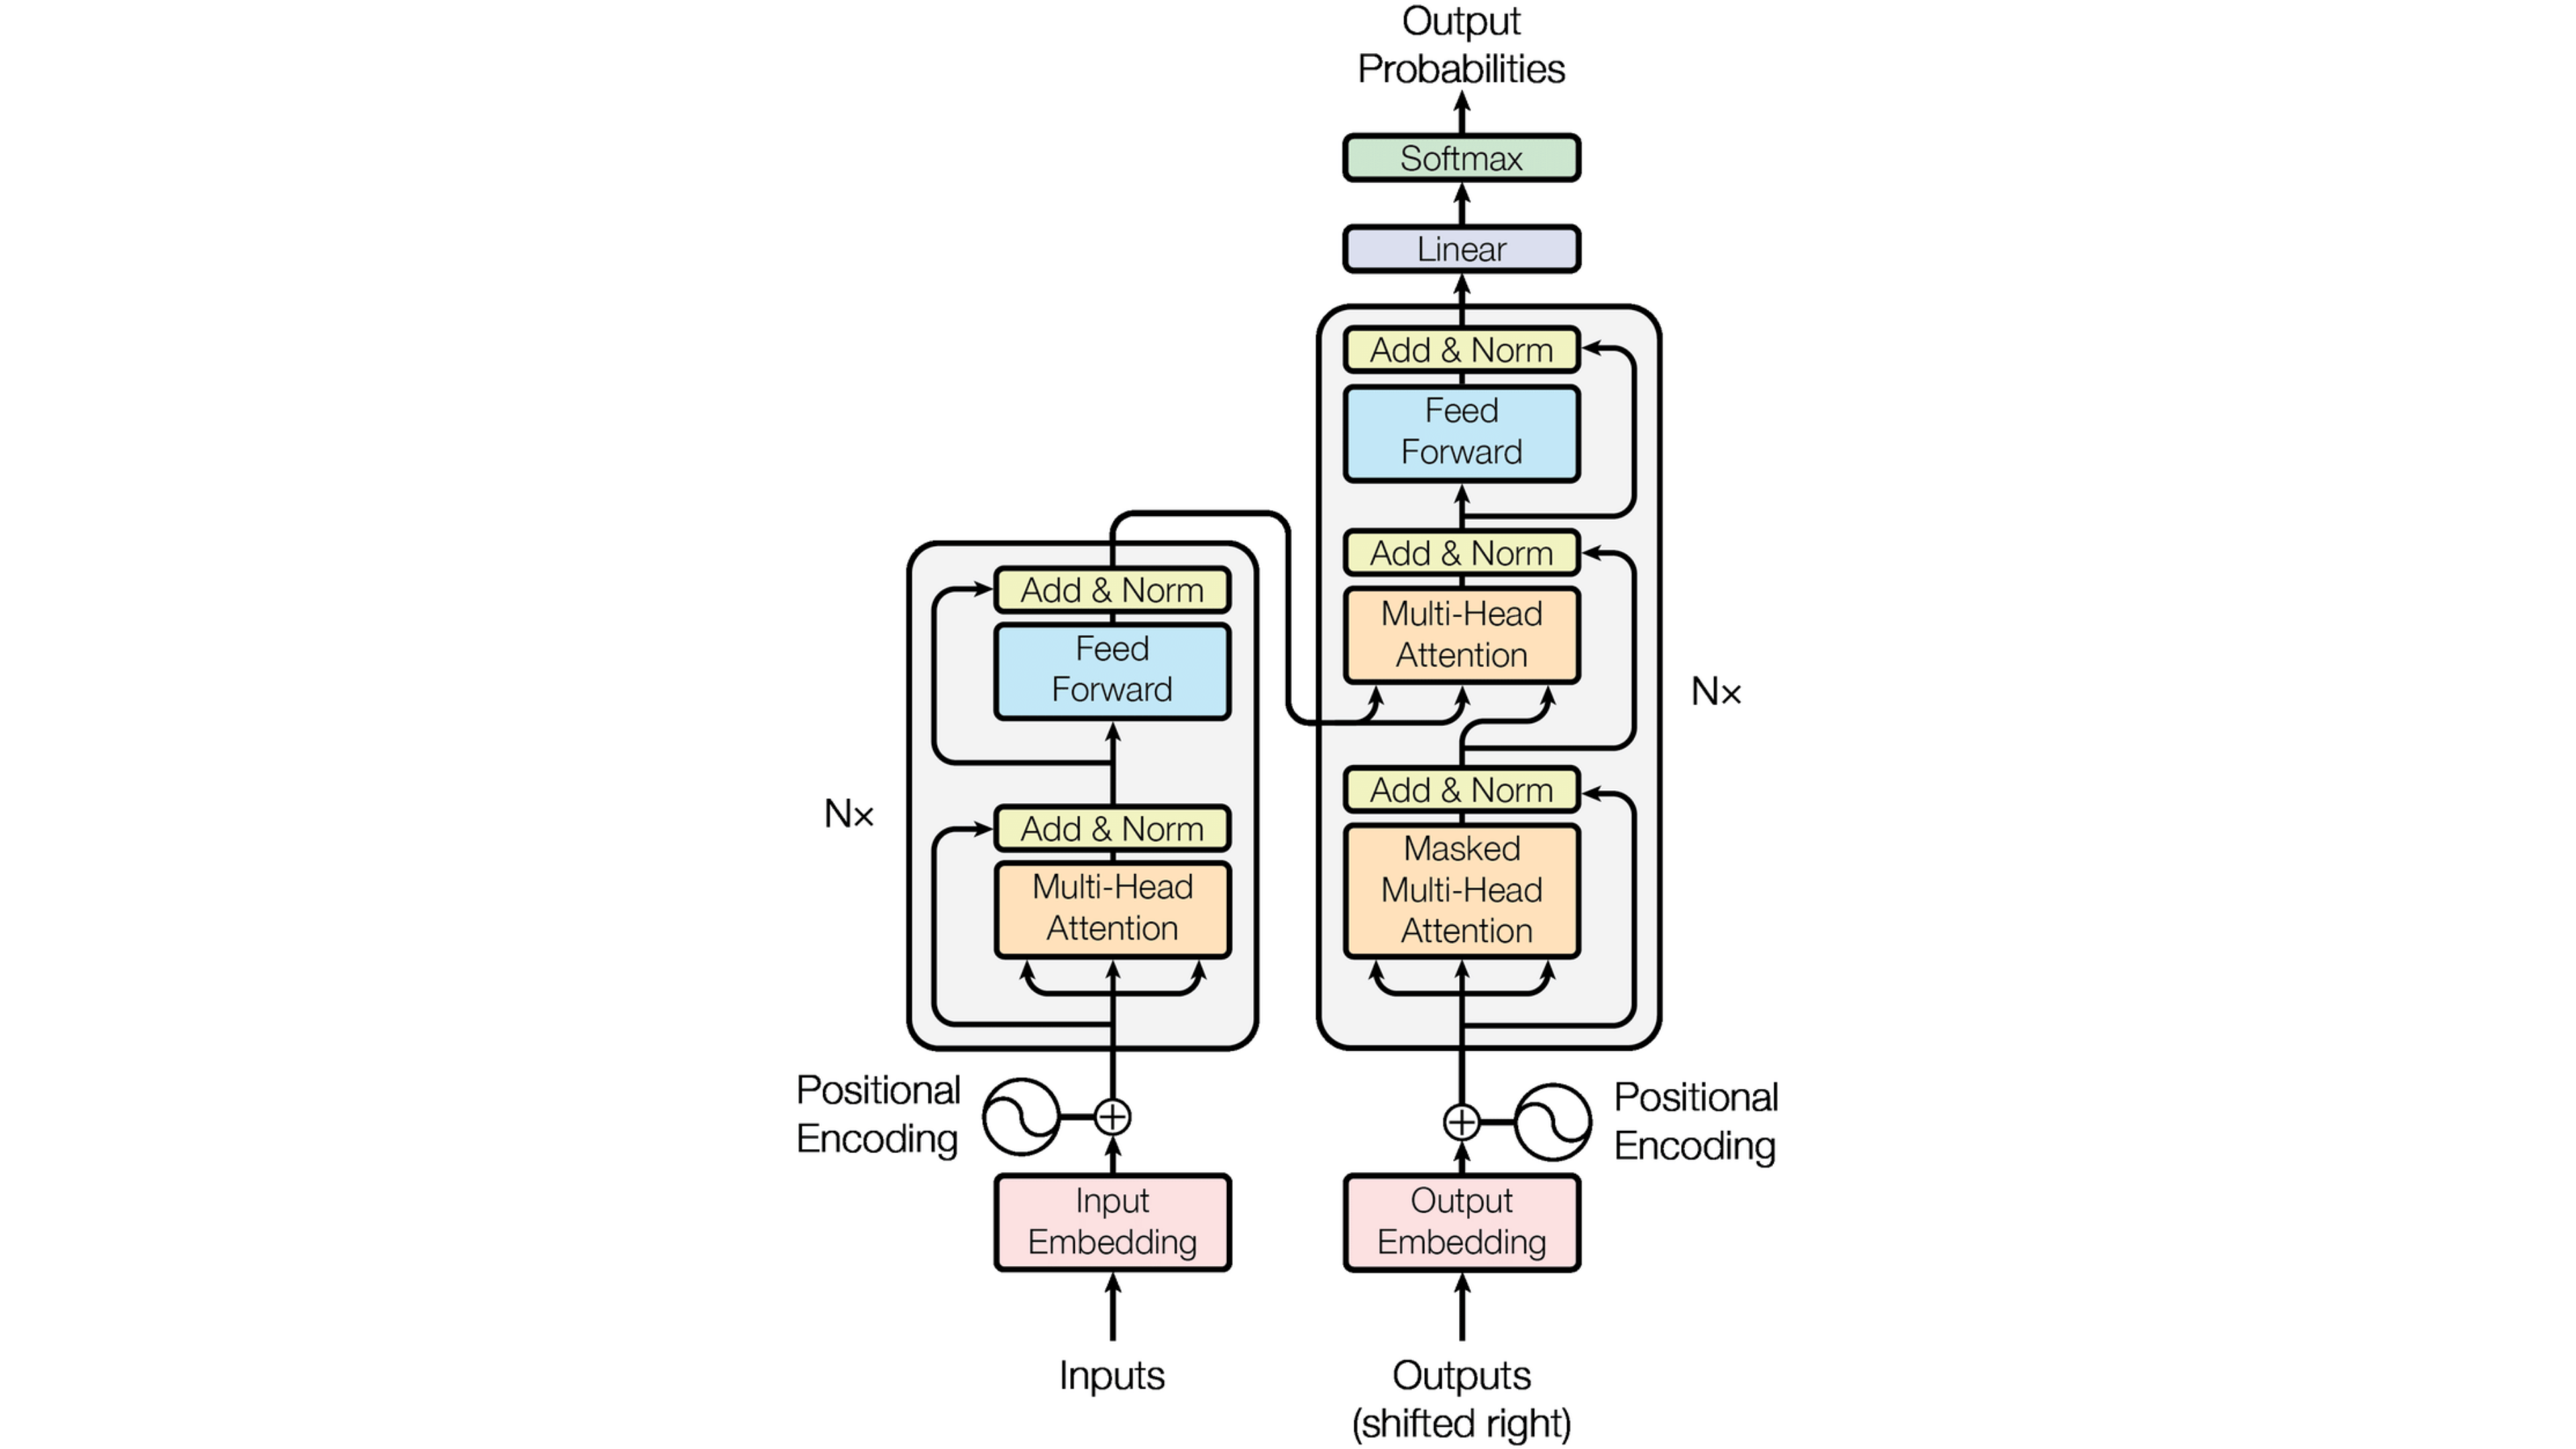
\includegraphics[width=1\textwidth]{Gambar/arch transformer.png}}
    \caption{Arsitektur Transformer \citep{NIPS2017_3f5ee243}}
    \label{fig:transformer-arch}
\end{figure}

Evolusi \textit{LLM} telah melahirkan dua paradigma utama, yaitu model \textit{encoder-only} seperti \textit{BERT} yang unggul dalam pemahaman kontekstual dan ekstraksi informasi \citep{devlin2019bertpretrainingdeepbidirectional}, serta model \textit{decoder-only} seperti keluarga \textit{GPT} yang dioptimalkan untuk tugas-tugas generatif \textit{autoregresif} \citep{Radford2018ImprovingLU}. Melalui proses \textit{pre-training} pada triliunan token data dari internet, buku, dan artikel ilmiah, \textit{LLM} menunjukkan fenomena \textit{emergent properties}, di mana kemampuan kompleks seperti penalaran \textit{chain-of-thought}, pemecahan masalah matematika, dan \textit{in-context learning} (ICL) muncul seiring dengan peningkatan skala parameter model \citep{brown2020languagemodelsfewshotlearners}. Kemampuan \textit{ICL} ini sangat krusial karena memungkinkan model beradaptasi dengan tugas baru melalui instruksi teks tanpa memerlukan pelatihan ulang (\textit{retraining}) yang mahal.

Pada tahap inferensi, \textit{LLM} menghasilkan token secara \textit{autoregresif} berdasarkan distribusi probabilitas bersyarat:
\begin{equation}
    y_t = \arg\max_{y} P_\theta(y \mid y_{<t}, x),
    \label{eq:llm-generation}
\end{equation}
di mana $y_t$ merupakan token yang dihasilkan pada langkah waktu $t$, yang ditentukan berdasarkan probabilitas bersyarat $P_\theta$ terhadap urutan token sebelumnya ($y_1$ hingga $y_{t-1}$) dan input $x$ yang diberikan.

Namun, terlepas dari kecanggihannya, \textit{LLM} memiliki keterbatasan fundamental yang menjadi tantangan besar dalam domain akademik. Model ini bersifat probabilistik, bukan mesin penalaran logis murni, yang berarti model menghasilkan teks berdasarkan tebakan statistik terhadap kelanjutan kata yang paling mungkin, bukan berdasarkan pemahaman fakta yang absolut. Studi oleh \cite{lála2023paperqaretrievalaugmentedgenerativeagent} menyebutkan bahwa hal ini menyebabkan munculnya halusinasi, di mana model memberikan jawaban yang terdengar meyakinkan namun salah secara faktual atau sepenuhnya fabrikasi. Selain itu, \textit{LLM} mengalami kendala \textit{knowledge cutoff}, di mana pengetahuan model terbatas pada data pelatihan terakhirnya, sehingga tidak mampu mengakses informasi terkini atau literatur ilmiah terbaru yang diterbitkan setelah masa pelatihannya.

Dalam penelitian ini, \textit{LLM} berperan sebagai ``otak'' atau unit pemrosesan utama dalam arsitektur sistem yang bertanggung jawab untuk menghasilkan jawaban. Oleh karena itu, mengintegrasikan \textit{LLM} dengan pengetahuan eksternal menjadi strategi penting untuk mengurangi risiko halusinasi dengan cara memberikan dasar (\textit{grounding}) pada setiap respons generatif menggunakan fakta terstruktur yang dapat diverifikasi dan memiliki jejak data (\textit{provenance}) yang jelas.

\subsection{\textit{Retrieval-Augmented Generation} (RAG)}

\textit{Retrieval-Augmented Generation (RAG)} adalah sebuah arsitektur yang dirancang untuk meningkatkan performa model bahasa besar (\textit{LLM}) dengan menggabungkan mekanisme pencarian informasi eksternal ke dalam proses generasi teks \citep{lewis2021retrievalaugmentedgenerationknowledgeintensivenlp}. Secara prinsip, \textit{RAG} berperan sebagai penghubung antara kemampuan penalaran linguistik statis dari \textit{LLM} dengan basis pengetahuan eksternal dinamis yang dapat diperbarui terus-menerus. Pendekatan ini menghasilkan konsep yang dikenal sebagai \textit{grounded intelligence} atau kecerdasan yang berlandaskan bukti, di mana model tidak hanya mengandalkan pengetahuan internalnya, tetapi juga melakukan pencarian pada dokumen referensi sebelum memberikan respons \citep{Huang_2025}.

Sebagaimana ditekankan oleh \citet{Huang_2025}, pendekatan ini dirancang secara efektif untuk memitigasi keterbatasan inheren pada \textit{LLM}, seperti fenomena halusinasi (\textit{hallucination}), keterbatasan pengetahuan akibat masa pelatihan yang statis (\textit{knowledge cutoff}), serta kurangnya spesialisasi pada domain tertentu. Dengan menyandarkan respons pada dokumen pendukung yang relevan, \textit{RAG} memungkinkan model untuk menghasilkan jawaban yang lebih akurat dan terverifikasi. Secara umum, alur kerja standar RAG terdiri dari tiga tahapan utama, yaitu:

\begin{enumerate}[label=\textbf{\Alph*.}, leftmargin=0.75cm]
    \item \textbf{\textit{Indexing}:} Segmentasi teks menjadi \textit{chunks} dan konversi ke representasi vektor (\textit{embedding}) dalam basis data.

    \item \textbf{\textit{Retrieval}:} Pencarian kemiripan semantik (\textit{semantic similarity}) untuk menemukan potongan teks relevan berdasarkan kueri pengguna.

    \item \textbf{\textit{Generation}:} Sintesis jawaban oleh \textit{LLM} menggunakan \textit{augmented prompt} yang menggabungkan kueri asli dan konteks yang ditemukan.
\end{enumerate}

Evolusi \textit{RAG} telah melahirkan berbagai paradigma. \cite{gao2024retrievalaugmentedgenerationlargelanguage} mengklasifikasikan evolusi metode \textit{RAG} ke dalam tiga paradigma utama. Pertama, \textbf{\textit{Naive RAG}} yang menggunakan pola \textit{retrieve-read} sederhana melalui kesamaan vektor. Kedua, \textbf{\textit{Advanced RAG}} yang menerapkan optimasi pra-pengambilan (seperti ekspansi kueri) dan pasca-pengambilan (seperti pemeringkatan ulang atau \textit{reranking}) untuk meningkatkan presisi hasil \citep{ma2023queryrewritingretrievalaugmentedlarge}. Selanjutnya, metode \textbf{\textit{Modular RAG}} menawarkan fleksibilitas melalui integrasi modul fungsional untuk pengolahan data terstruktur seperti grafik atau tabel \citep{Wang2023KnowledGPTEL}. Secara garis besar, paradigma-paradigma metode tersebut diilustrasikan pada \ref{fig:rag-process}.

\begin{figure}[!t]
    \centering
    \makebox[\textwidth][c]{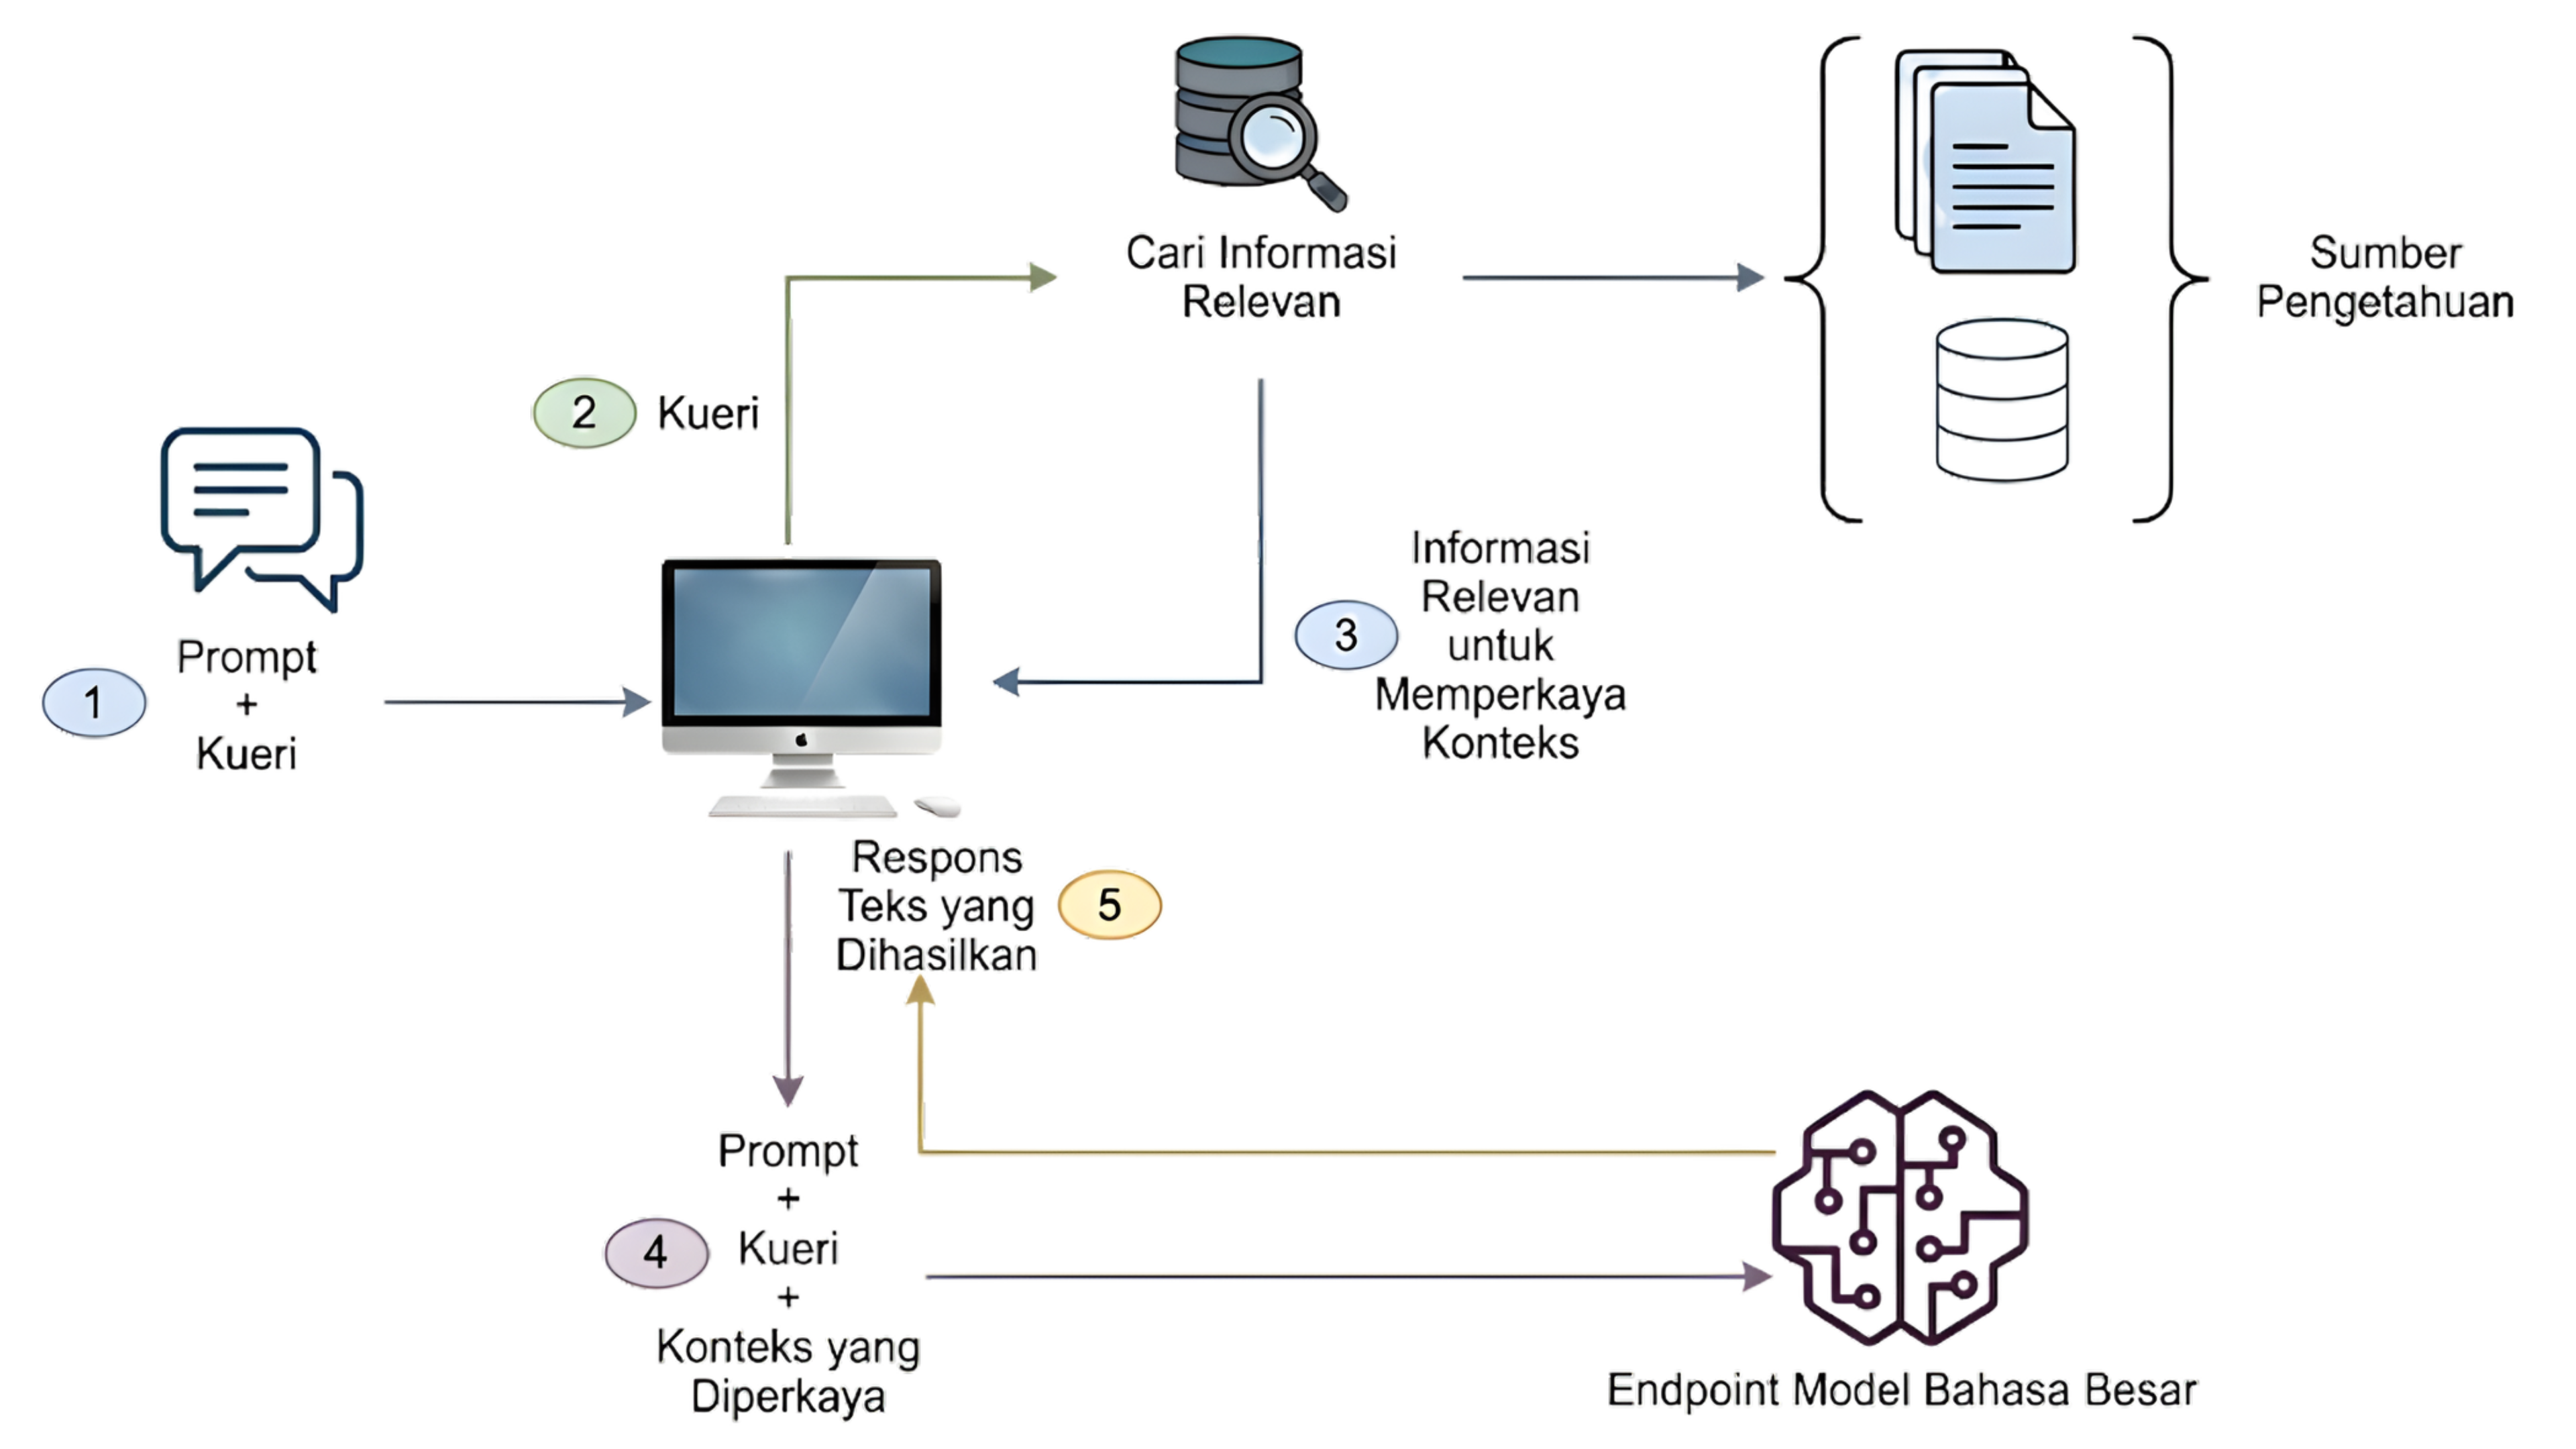
\includegraphics[width=1\textwidth]{Gambar/rag new.png}}
    \caption{Diagram Alur \textit{Retrieval-Augmented Generation} (RAG)}
    \label{fig:rag-process}
\end{figure}

Berbagai penelitian telah dilakukan untuk mengembangkan sistem \textit{RAG}. Penelitian oleh \cite{luan2021sparsedenseattentionalrepresentations} melakukan studi pengembangan metode \textit{Information Retrieval} pada \textit{RAG} dan menemukan bahwa metode tersebut seringkali tidak dapat menemukan informasi relevan apabila pertanyaan bersifat kompleks. Penelitian terkini juga menunjukkan bahwa penggunaan satu metode pengambilan informasi kurang efektif. Mulai berkembang penelitian yang menggabungkan dua pendekatan yaitu pencarian berbasis kata kunci (\textit{sparse retrieval}) dan pencarian berdasarkan makna atau konteks (\textit{dense retrieval}). Penggabungan metode ini memungkinkan sistem mengambil informasi yang relevan meskipun penggunaan istilah berbeda tetapi memiliki makna serupa.

Namun, implementasi \textit{RAG} konvensional yang hanya berbasis pada kemiripan vektor (\textit{Vector RAG}) sering menghadapi tantangan berupa fragmentasi konteks, di mana hubungan antar-dokumen yang kompleks atau struktur hierarkis dalam literatur akademik cenderung terabaikan. Keterbatasan dalam melakukan penalaran pencarian pada data yang saling terkait inilah yang mendorong perlunya integrasi struktur data yang lebih kaya dan dapat membaca hubungan antar-dokumen yang kompleks.

\subsection{\textit{Graph-Based RAG}}

\textit{Graph-Based Retrieval-Augmented Generation} (GraphRAG) merupakan evolusi dari paradigma \textit{RAG} konvensional yang mengintegrasikan pengetahuan terstruktur dari \textit{Knowledge Graph} ke dalam mekanisme \textit{retrieval} model bahasa besar \citep{peng2024graphretrievalaugmentedgenerationsurvey}. Berbeda dengan \textit{Vector RAG} tradisional yang hanya mengandalkan potongan teks (\textit{chunks}) terfragmentasi berdasarkan kemiripan vektor, \textit{GraphRAG} secara khusus mengekstraksi hubungan eksplisit antar entitas untuk memperkaya konteks yang akan diberikan kepada model bahasa \citep{guo2023gpt4graphlargelanguagemodels}. Pendekatan ini secara mendasar mengubah cara mesin melakukan navigasi pengambilan informasi dari sekadar mencari ``kata-kata yang mirip'' menjadi proses penalaran relasional yang mampu menghubungkan poin-poin data yang tersebar di berbagai dokumen.

\begin{figure}[!t]
    \centering
    \makebox[\textwidth][c]{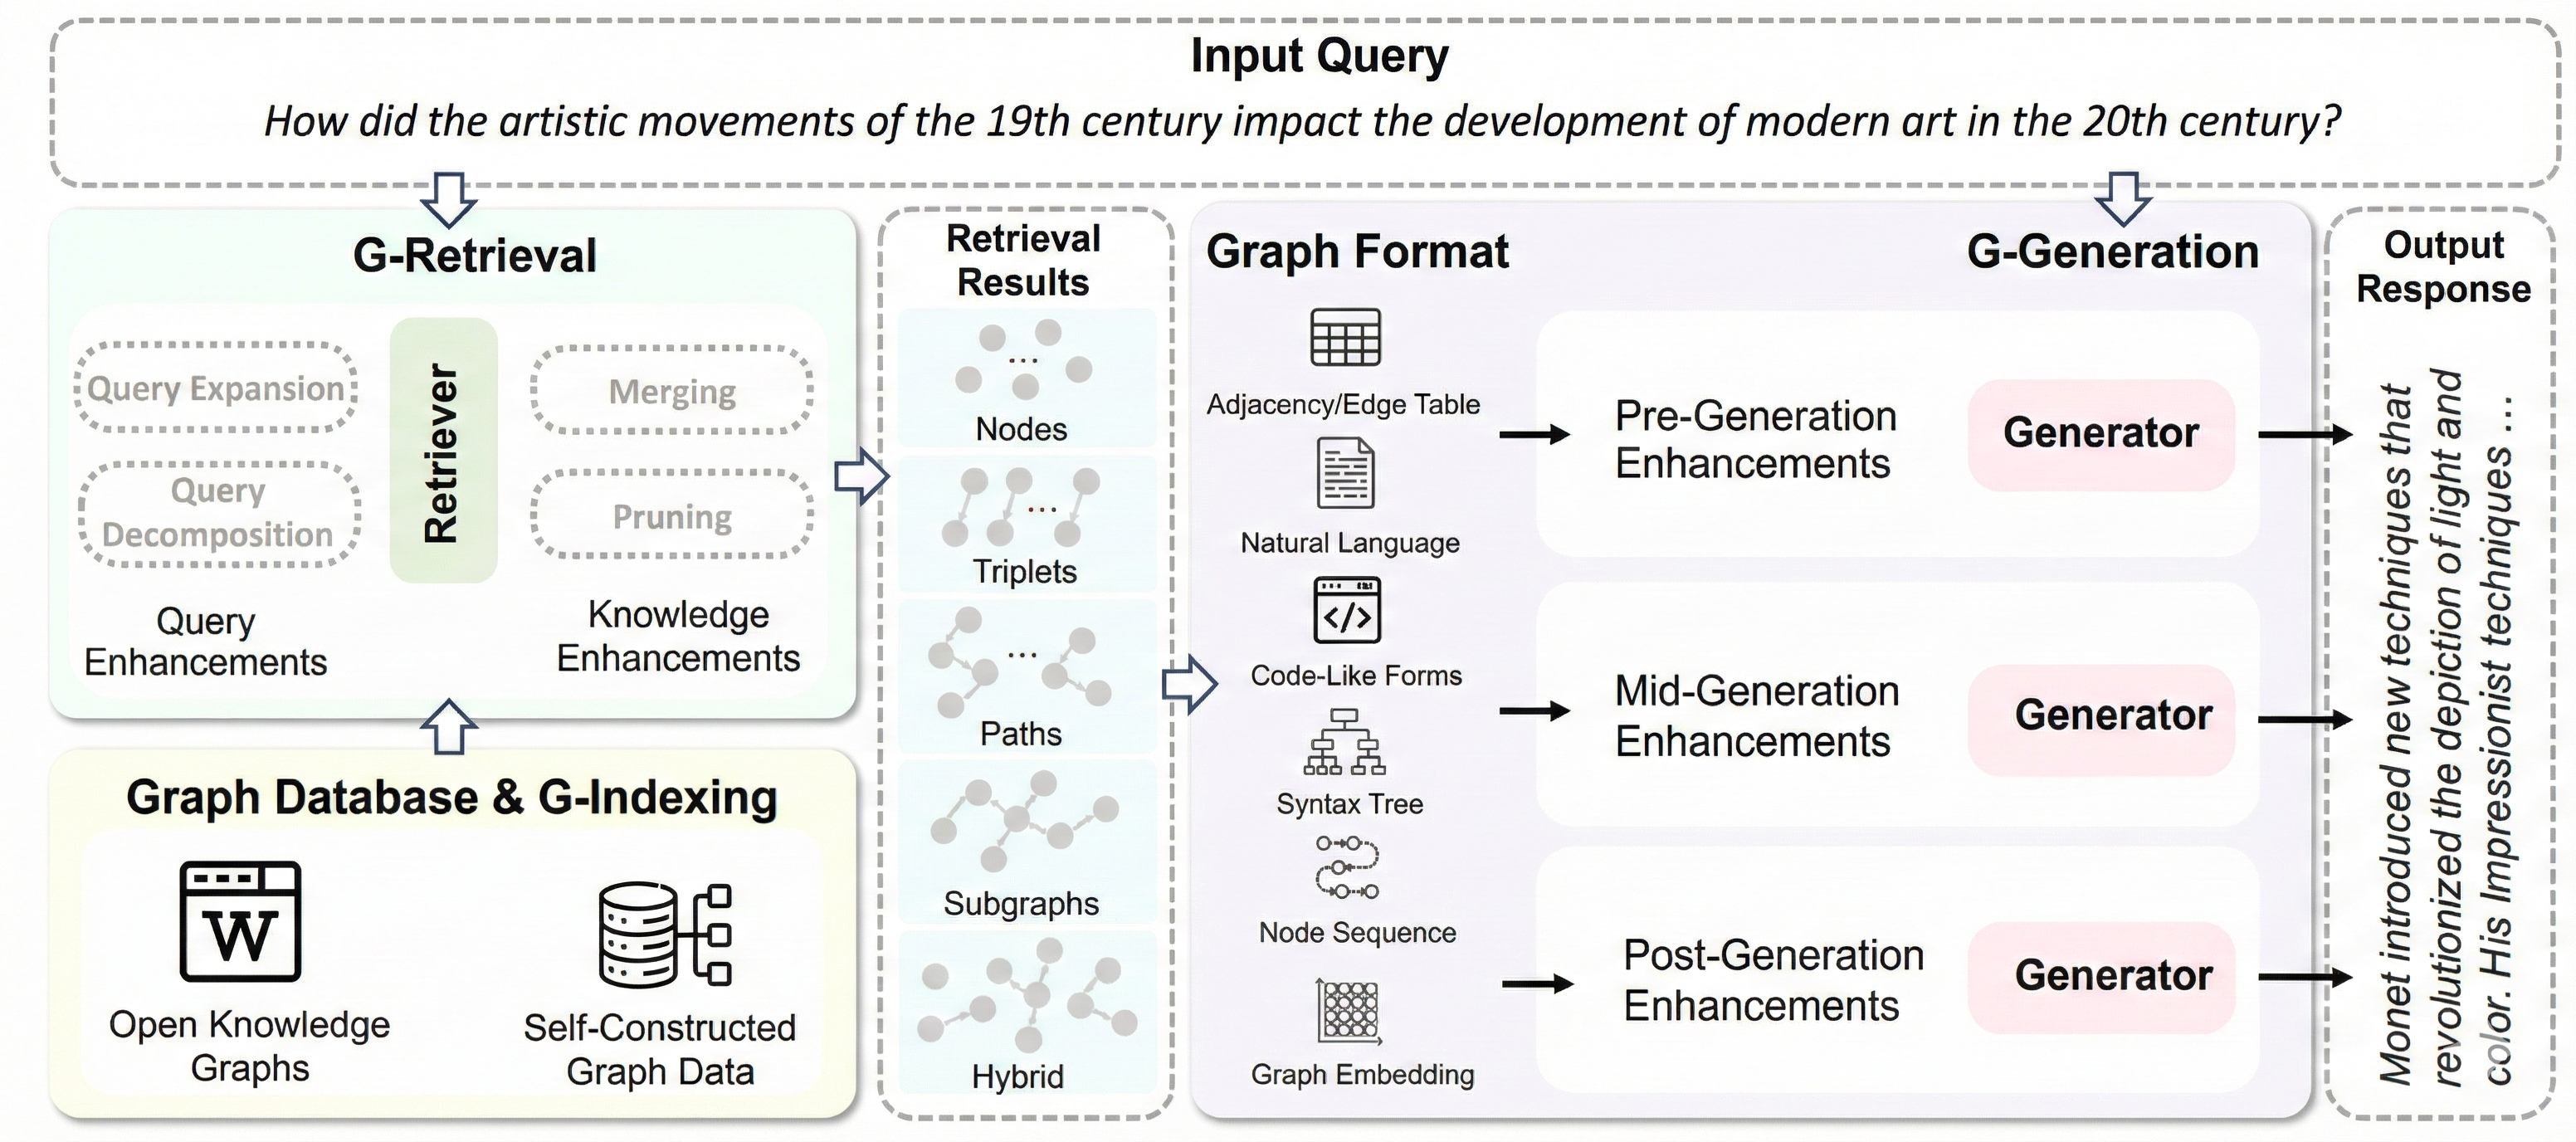
\includegraphics[width=1\textwidth]{Gambar/framework graphrag.png}}
    \caption{Alur Graph-Based RAG untuk tugas \textit{Question-Answering}
        \citep{peng2024graphretrievalaugmentedgenerationsurvey}}
    \label{fig:graphrag-framework}
\end{figure}

Tujuan \textit{GraphRAG} adalah menemukan jawaban optimal ($a^*$) untuk pertanyaan ($q$) berbasis Graf Pengetahuan ($\mathcal{G}$), diformulasikan sebagai:

\begin{equation}
    a^* = \operatorname*{arg\,max}_{a \in A} p(a|q, \mathcal{G})
    \label{eq:graphrag_goal}
\end{equation}
di mana \(A\) merepresentasikan himpunan seluruh kemungkinan respons yang dapat dihasilkan. Untuk mencapai tujuan tersebut, distribusi probabilitas target \(p(a \mid q, \mathcal{G})\) dimodelkan melalui kolaborasi dua komponen utama, yaitu model \textit{graph retriever} \(p_\theta(G \mid q, \mathcal{G})\) dan model \textit{answer generator} \(p_\phi(a \mid q, G)\), di mana \(\theta\) dan \(\phi\) adalah parameter yang dapat dilatih.

\begin{equation}
    p(a \mid q, \mathcal{G}) \approx p_\phi(a \mid q, G^*)\, p_\theta(G^* \mid q, \mathcal{G})
    \label{eq:graphrag_decomposition_approx}
\end{equation}
Di sini, $p_\theta$ mewakili parameter model \textit{retriever} yang mencari subgraf relevan, sementara $p_\phi$ adalah model \textit{generator} yang menyusun jawaban berdasarkan subgraf tersebut.

Secara arsitektural, implementasi \textit{GraphRAG} terbagi menjadi tiga tahapan utama, sebagaimana diilustrasikan pada \ref{fig:graphrag-framework}:

\begin{enumerate}[label=\textbf{\Alph*.}, leftmargin=0.75cm]
    \item \textbf{Graph-Based Indexing (G-Indexing):} Tahap pembangunan basis data graf terstruktur yang berfungsi sebagai sumber pengetahuan. Proses ini mengorganisir entitas (\textit{nodes}) dan relasi (\textit{edges}) sedemikian rupa untuk mengoptimalkan pencarian. Data graf ini dapat berasal dari sumber terbuka seperti Wikidata \citep{wikidata} atau dibangun secara mandiri dari kumpulan dokumen akademik tertentu. Indeksasi adalah tahap paling krusial karena menentukan seberapa detail informasi yang dapat diambil nantinya.

    \item \textbf{Graph-Guided Retrieval (G-Retrieval):} Pada tahap pengambilan, sistem bertujuan mengambil elemen graf yang paling relevan, seperti pasangan subjek-predikat-objek (\textit{triples}), jalur hubungan (\textit{paths}), atau subgraf utuh, yang dapat diformulasikan sebagai:
          \begin{align}
              G^{*} & = \mathbf{G\text{-}Retriever}(q, G) \notag                                        \\
                    & = \arg\max_{G \subseteq \mathcal{R}(G)} p_{\theta}(G|q, G) \notag                 \\
                    & = \arg\max_{G \subseteq \mathcal{R}(G)} \mathbf{Sim}(q,G), \label{eq:g-retrieval}
          \end{align}

    \item \textbf{Graph-Enhanced Generation (G-Generation):} Pada tahap generasi, data graf yang diambil diintegrasikan ke dalam proses pembuatan jawaban. Struktur graf ini dapat diubah menjadi teks naratif atau diproses langsung oleh model \textit{transformer} yang peka terhadap struktur graf agar menghasilkan respons yang koheren, informatif, dan valid, yang dapat dinotasikan sebagai:
          \begin{align}
              a^{*} & = \mathbf{G\text{-}Generator}(q,G^{*}) \notag                                         \\
                    & = \arg\max_{a \in \mathcal{A}} p_{\phi}(a|q,G^{*}) \notag                             \\
                    & = \arg\max_{a \in \mathcal{A}} p_{\phi}(a|\text{F}(q,G^{*})), \label{eq:g-generation}
          \end{align}
\end{enumerate}


Salah satu inovasi penting dalam domain ini adalah kerangka kerja \textit{Microsoft GraphRAG}, yang memperkenalkan konsep deteksi komunitas hierarkis dengan menggunakan algoritma \textit{Leiden} \citep{edge2025localglobalgraphrag}. Metode ini membagi graf menjadi klaster-klaster yang kemudian diringkas menjadi laporan komunitas (\textit{community reports}), sehingga memungkinkan sistem untuk menjawab kueri bersifat ``global'' (tema besar dalam satu dataset) yang biasanya gagal ditangani oleh \textit{RAG} berbasis vektor. Namun, pendekatan ini menghadapi tantangan seperti tingginya biaya komputasi dan risiko cakupan komunitas yang terlalu luas saat skala data bertambah besar. Sebagai perbaikan, pendekatan \textit{LightRAG} memitigasi hal ini dengan mekanisme pengambilan dua tingkat menggunakan kata kunci \textit{lokal} dan \textit{global} \citep{guo2025lightragsimplefastretrievalaugmented}. Teknik ini secara signifikan mengurangi beban komputasi serta dipercaya dapat mempercepat pencarian. Namun, penerapan metode ini masih jarang dilakukan di lingkungan akademik yang berisiko mengalami hilangnya hubungan antar entitas jika tidak dipetakan secara eksplisit.

Merespons keterbatasan masing-masing pendekatan tersebut, penelitian ini menerapkan strategi \textit{Hybrid Vector-Graph Retrieval} untuk mengoptimalkan kinerja sistem. Pendekatan hibrida ini diperlukan untuk menyinergikan keunggulan metode pengambilan informasi konvensional berbasis \textit{semantic retrieval} (vektor) yang cepat dalam pencarian kemiripan, dengan \textit{structured retrieval} (graf) yang unggul dalam penalaran relasional. Sinergi ini dirancang untuk menyeimbangkan antara efisiensi komputasi dan akurasi kontekstual, sehingga sistem mampu menyajikan referensi ilmiah yang relevan dan mendalam tanpa menimbulkan \textit{bottleneck} dalam proses \textit{inference}.